\documentclass[12pt,a4paper]{article}
\usepackage[utf8]{vietnam}
\usepackage{amsmath}
\usepackage{amsfonts}
\usepackage{amssymb}
\usepackage{graphicx}
\usepackage[left=2cm,right=2cm,top=2cm,bottom=2cm]{geometry}
\usepackage{indentfirst}
\usepackage{chngcntr}
\counterwithin{figure}{section}
\counterwithin{table}{section}
\counterwithin{equation}{section}
\usepackage{fancyhdr}
\pagestyle{fancy}
\fancyhf{}
\rhead{GVHD: Nguyễn Lý Thiên Trường}
\lhead{Đồ án môn học}
\rfoot{Trang \thepage}
\usepackage{cases} 
\usepackage{listings}
\usepackage{color}
\definecolor{dkgreen}{rgb}{0,0.6,0}
\definecolor{gray}{rgb}{0.5,0.5,0.5}
\definecolor{mauve}{rgb}{0.58,0,0.82}
\lstset{frame=tb,
      language=Python,
      aboveskip=3mm,
      belowskip=3mm,
      showstringspaces=false,
      columns=flexible,
      basicstyle={\small\ttfamily},
      numbers=none,
      numberstyle=\tiny\color{gray},
      keywordstyle=\color{blue},
      commentstyle=\color{dkgreen},
      stringstyle=\color{mauve},
      breaklines=true,
      breakatwhitespace=true,
      tabsize=3
    } 
\begin{document}
\setcounter{page}{1}
\pagenumbering{roman}
\section*{LỜI CẢM ƠN}
Cảm ơn thầy Nguyễn Lý Thiên Trường đã hướng dẫn em hoàn thành đồ án này. Nhờ có sự chỉ dẫn nhiệt tình của thầy, em đã học được cách phân tích và giải quyết từng vấn đề trong quá trình thực hiện đồ án.

\begin{flushright}
Thành phố Hồ Chí Minh, ngày 25 tháng 5 năm 2019 
\end{flushright} 
\pagebreak
\section*{TÓM TẮT}
Đồ án này trình bày về việc xây dựng một chương trình để phát hiện và phân loại trái Sơri sử dụng các giải thuật máy học cơ bản và bộ thư viện mã nguồn mở OpenCV trên ngôn ngữ Python.

Đầu tiên chương trình sẽ sử dụng thuật toán Haar Cascade để xác định vùng chứa trái Sơri, sau đó sử dụng thuật toán K-láng giềng gần nhất (K-NN) để dự đoán xem đó là trái Sơri xanh hay chín.
 
\pagebreak
\tableofcontents
\pagebreak
\listoffigures
\pagebreak
\listoftables
\pagebreak
\setcounter{page}{1}
\pagenumbering{arabic}
\section{GIỚI THIỆU}
\subsection{Tổng quan}
Máy học và thị giác máy tính là những chuyên ngành được phát triển khá lâu và có nhiều ứng dụng rộng rãi trong đời sống như: Tìm kiếm vật thể trong ảnh, nhận diện khuôn mặt, đọc biển số xe, nhận diện dấu vân tay,...Trong nông nghiệp: Phân loại rau củ quả, phát hiện bệnh trên các loại quả,...
\begin{center}
    \begin{figure}[htp]
    \begin{center}
    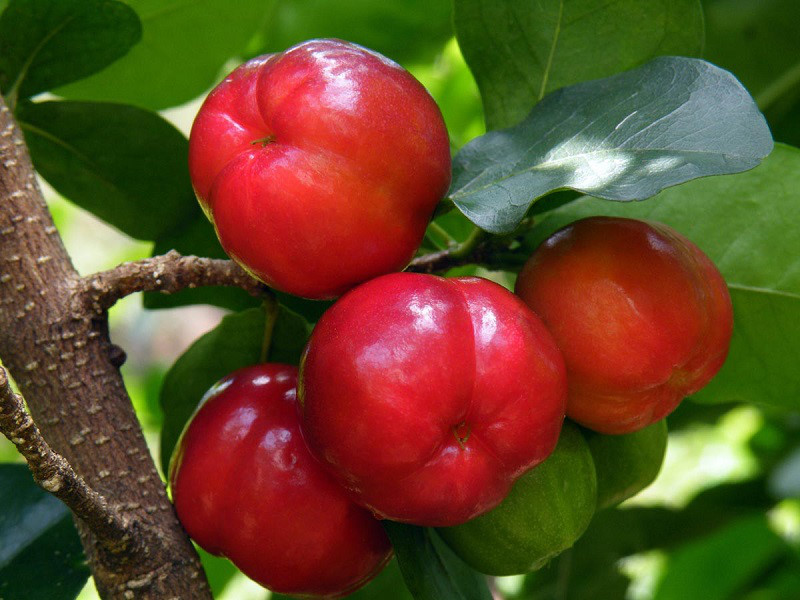
\includegraphics[scale=.2]{Images/sori}
    \end{center}
    \caption{Trái Sơri}
    \end{figure}
\end{center}
Trái Sơri (hay Acerola) là loại quả mọng, vỏ nhẵn bóng và có vị ngọt, với hàm lượng Vitamin C gấp 20-40 lần cam, chanh. Sơri còn chứa nhiều vi chất tốt cho sức khỏe như A, K, E, B1, B2, B3, B6, B12, sắt, magie, kali, canxi, kẽm, phospho, chất xơ, các axit amin và một số axit béo....Trái có hình tròn, khi chín có màu đỏ. Hiện nay ở khu vực Gò Công - Tiền Giang, diện tích canh tác cây Sơri khá lớn do phù hợp về thổ nhưỡng và khí hậu, góp phần không nhỏ vào việc ổn định kinh tế cho bà con nông dân. Tuy nhiên quá trình thu hoạch và các công đoạn sau thu hoạch còn tốn nhiều thời gian (do phải làm thủ công) dẫn đến hiệu quả kinh tế còn chưa cao.
\subsection{Nhiệm vụ đề tài}
Nhiệm vụ đặt ra ở đồ án này là ứng dụng các thuật toán máy học đơn giản để xây dựng mô hình phần mềm phân loại trái Sơri theo màu sắc (xanh và chín) với độ chính xác cao, thời gian trễ thấp, là bước đầu để xây dựng hoàn chỉnh hệ thống phân loại trái Sơri. 
\section{LÝ THUYẾT}
\subsection{Thuật toán Haar Cascade [1]}
Haar Cascade là một thuật toán trong máy học dùng để xác định các đối tượng trong hình ảnh hoặc video dựa trên các đặc trưng được đề xuất bởi Paul Viola và Michael Jones (2001). Thuật toán gồm 4 giai đoạn:
\begin{itemize}
\item[-] Lựa chọn các đặc trưng Haar
\item[-] Tính Integral Images
\item[-] Huấn luyện Adaboost
\item[-] Thực hiện mô hình phân tầng Cascade
\end{itemize} 
\subsubsection{Đặc trưng Haar-like}
Đặc trưng Haar-like được tạo thành bằng việc kết hợp các hình chữ nhật đen, trắng với nhau theo một trật tự, một kích thước nào đó. Có 4 đặc trưng Haar-like cơ bản:
\begin{center}
    \begin{figure}[htp]
    \begin{center}
    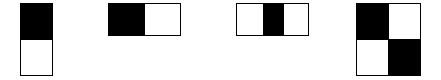
\includegraphics[scale=.7]{Images/Haarlike}
    \end{center}
    \caption{4 đặc trưng cơ bản}
    \end{figure}
\end{center}
Ngoài ra còn có các đặc trưng mở rộng:
\begin{center}
    \begin{figure}[htp]
    \begin{center}
    
\includegraphics[scale=.7]{Images/edgefeature}
    \end{center}
    \caption{Đặc trưng cạnh}
    \end{figure}
\end{center}
\begin{center}
    \begin{figure}[htp]
    \begin{center}
    
\includegraphics[scale=.7]{Images/linefeature}
    \end{center}
    \caption{Đặc trưng đường}
    \end{figure}
\end{center}
Ứng với mỗi đặc trưng, một bộ phân lớp yếu $h_k(x)$ được định nghĩa như sau:
\begin{subnumcases}{h_k(x) = }
    1 & $ p_kf_k(x) < p_k\theta_k$ \\
	0 & $ else $    
\end{subnumcases}
Trong đó:
\begin{itemize}
\item x: cửa sổ con cần xét.
\item $\theta_k$: ngưỡng.
\item $f_k$: giá trị của đặc trưng Haar-Like.
\item $p_k$: hệ số  quyết định chiều của bất phương trình.
\end{itemize}
Ta hiểu công thưc trên đơn giản như sau: Khi giá trị của đặc trưng Haar-Like k $f_k$ tại cửa sổ con x vượt qua một ngưỡng $\theta_k$ thì một bộ phân lớp $h_k(x)$ sẽ kết luận cửa sổ con x là trái Sơri, còn $f_k$ không vượt qua ngưỡng đó thì không là trái Sơri. Ngưỡng $\theta_k$ là giá trị rút ra sau quá trình huấn luyện bộ phân lớp, sẽ trình bày sau.
\pagebreak
\subsubsection{Tính Integral Image}
Gía trị của đặc trưng Haar-like là sự chênh lệch giữa tổng các điểm ảnh của các vùng đen và các vùng trắng. Để tính nhanh các đặc trưng này, Viola và Jones đã giới thiệu khái niệm ảnh tích phân (Integral Image). Integral Image là một mảng hai chiều với kích thước bằng kích thước của ảnh cần tính đặc trưng Haar-like.
\begin{center}
    \begin{figure}[htp]
    \begin{center}
    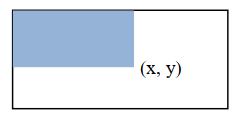
\includegraphics[scale=.7]{Images/integral}
    \end{center}
    \caption{Tính giá trị ảnh tích phân tại điểm có tọa độ (x, y)}
    \end{figure}
\end{center}
Gía trị ảnh tích phân tại điểm P có tọa độ (x, y) được tính như sau:
\begin{equation}
    P(x, y) = \sum_{x' \leqslant x, y' \leqslant y} i(x', y')
\end{equation}
Sau khi đã tính được ảnh tích phân , việc tính tổng các giá trị mức xám của một vùng ảnh bất kỳ nào trên ảnh được thực hiện như sau.
\begin{center}
    \begin{figure}[htp]
    \begin{center}
    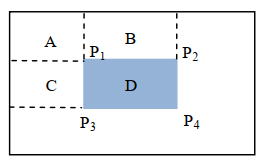
\includegraphics[scale=.7]{Images/integral1}
    \end{center}
    \caption{Ví dụ tính tổng các giá trị mức xám trên vùng D}
    \end{figure}
\end{center}
Gỉa sử ta cần tính tổng các giá trị mức xám của vùng D như trong hình  2.6 ta có thể tính như sau:
\begin{equation}
    D = A + B + C + D - (A + B) - (A + C) + A
\end{equation}
Hay
\begin{equation}
	D = P4 + P1 - (P2 + P3)
\end{equation}
\pagebreak
\subsubsection{Thuật toán Adaboost}
AdaBoost là một bộ phân loại mạnh phi tuyến phức, hoạt động dựa trên nguyên tắc kết hợp tuyến tính các bộ phân loại yếu để tạo nên một bộ phân loại mạnh. AdaBoost sử dụng trọng số để đánh dấu các mẫu khó nhận dạng. Trong quá trình huấn luyện cứ mỗi bộ phân loại yếu được xây dựng thì thuật toán sẽ tiến hành cập nhật lại trọng số để chuẩn bị cho việc xây dựng bộ phân loại tiếp theo. Cập nhật bằng cách tăng trọng số của các mẫu nhận dạng sai và giảm trọng số của các mẫu được nhận dạng đúng bởi bộ phân loại yếu vừa xây dựng. Bằng cách này thì bộ phân loại sau có thể tập trung vào các mẫu mà bộ phân loại trước nó làm chưa tốt. Cuối cùng các bộ phân loại yếu sẽ được kết hợp lại tùy theo mức độ tốt của chúng để tạo nên một bộ phân loại mạnh.

Để trực quan hơn, ta hãy quan sát qua chuỗi hình ảnh sau:
\begin{center}
    \begin{figure}[htp]
    \begin{center}
    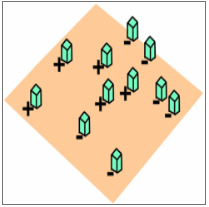
\includegraphics[scale=0.8]{Images/1}
    \end{center}
    \caption{Khởi tạo trọng số cho các mẫu}
    \end{figure}
\end{center}
\begin{center}
    \begin{figure}[htp]
    \begin{center}
    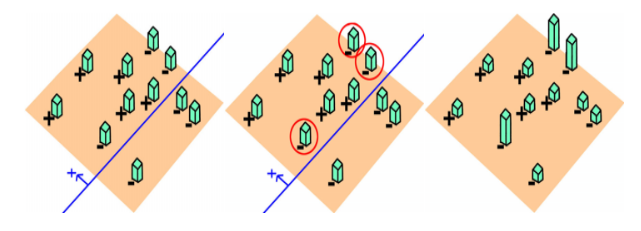
\includegraphics[scale=0.8]{Images/2}
    \end{center}
    \caption{Vòng lặp thứ 1}
    \end{figure}
\end{center}
\begin{center}
    \begin{figure}[htp]
    \begin{center}
    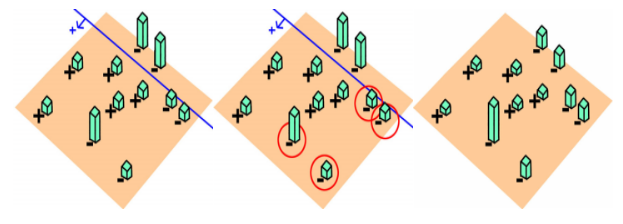
\includegraphics[scale=0.8]{Images/3}
    \end{center}
    \caption{Vòng lặp thứ 2}
    \end{figure}
\end{center}
\begin{center}
    \begin{figure}[htp]
    \begin{center}
    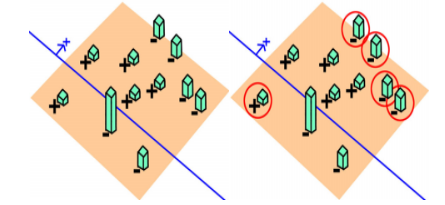
\includegraphics[scale=0.8]{Images/4}
    \end{center}
    \caption{Vòng lặp thứ 3}
    \end{figure}
\end{center}
\begin{center}
    \begin{figure}[htp]
    \begin{center}
    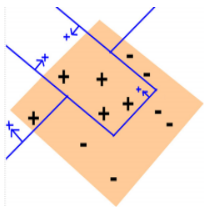
\includegraphics[scale=0.8]{Images/5}
    \end{center}
    \caption{Kết hợp các bộ phân loại yếu lại}
    \end{figure}
\end{center}
\pagebreak
\subsubsection{Mô hình phân tầng Cascade}
\begin{center}
    \begin{figure}[htp]
    \begin{center}
    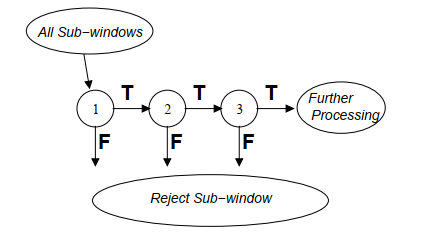
\includegraphics[scale=0.8]{Images/Cas}
    \end{center}
    \caption{Mô hình phân tầng Cascade}
    \end{figure}
\end{center}

Mẫu đầu vào được đưa vào bộ phân loại đầu tiên, nếu kết quả là True (có vật thể) thì nó sẽ được đưa qua bộ phân loại thứ 2 và tiếp tục như vậy đến cuối cùng nếu vượt qua hết các bộ phân loại thì kết quả tổng hợp sẽ là True. Nếu kết quả là False (không có vật thể) ở bất kỳ bộ phân loại nào thì nó sẽ cho kết quả tổng hợp là False ngay lập tức.

Như đã đề cập ở phần 2.1.1, giá trị ngưỡng quyết định ở mỗi bộ phân loại là kết quả của quá trình huấn luyện được mô tả như sau:
\begin{itemize}
\item Gỉa sử ta có 2 tập ảnh dương (có vật thể) và ảnh âm (không có vât thể).
\item Đầu tiên ta quy định số lượng bộ phân loại cần thực hiện.
\item Ở mỗi bộ phân loại ta đưa vào một số lượng ảnh dương và số lượng đặc trưng Haar bất kỳ. Chương trình sẽ tính toán ra tỉ lệ nhận dạng thành công, tỉ lệ nhận dạng sai và các đặc trưng thu được. Sau đó chương trình sẽ tăng số lượng đặc trưng Haar rồi cập nhật lại các giá trị tỉ lệ. Liên tục như vậy cho đến khi tỉ lệ nhận dạng đúng và sai bằng nhau (đây chính là giá trị ngưỡng) thì chuyển sang bộ phân loại kế tiếp.
\end{itemize} 
\pagebreak
\subsubsection{Hệ thống xác định vị trí vật thể}
Trong hình 2.12, từ ảnh gốc ban đầu ta sẽ tính được Integral Image, mục đích là để tính nhanh tổng của các giá trị mức xám của một vùng hình chữ nhật bất kỳ trên ảnh gốc. Các vùng ảnh con này sẽ được đưa qua các hàm Haar cơ bản để ước lượng đặc trưng, kết quả ước lượng sẽ được đưa qua bộ điều chỉnh AdaBoost để loại bỏ nhanh các đặc trưng không có khả năng là đặc trưng của quả Sơri. Chỉ có một tập nhỏ các đặc trưng mà bộ điều chỉnh AdaBoost cho là có khả năng là đặc trưng của quả Sơri mới được chuyển sang cho bộ quyết định kết quả. Bộ quyết định sẽ tổng hợp kết quả là quả Sơri nếu kết quả của các bộ phân loại yếu trả về là quả Sơri.
\begin{center}
    \begin{figure}[htp]
    \begin{center}
    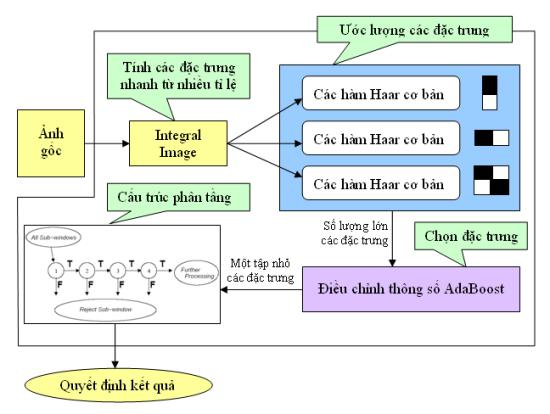
\includegraphics[scale=.8]{Images/class}
    \end{center}
    \caption{Hệ thống xác định vị trí vật thể}
    \end{figure}
\end{center}
\newpage
\subsection{Hệ màu RGB}
Hệ màu RGB là viết tắt của 3 màu cơ bản là Red, Green và Blue là ba màu chính của ánh sáng trắng sau khi được tách ra nhờ lăng kính. Những màu này khi kết hợp theo tỉ lệ nhất định sẽ tạo ra rất nhiều màu khác nhau trong dải ảnh sáng nhìn thấy, và khi kết hợp cả 3 màu lại với nhau với tỉ lệ 1 : 1 : 1 chúng ta sẽ được màu trắng. Bởi thế hầu hết các thiết bị điện tử sử dụng màu bằng cách phát quang như TV, màn hình máy tính, màn hình điện thoại… đều sử dụng RGB làm hệ màu chính. Và đó cũng là lý do mà các ảnh kỹ thuật số hiển thị trên máy tính đều sử dụng hệ RGB làm chuẩn.
\begin{center}
    \begin{figure}[htp]
    \begin{center}
    
\includegraphics[scale=.1]{Images/RGB}
    \end{center}
    \caption{Hệ màu RGB}
    \end{figure}
\end{center}
\subsection{Thuật toán ``K-Láng giềng gần nhất'' (K-NN) [6]}
K-Nearest Neighbours (K-NN)là một trong những thuật toán máy học đơn giản nhất.K-NN là phương pháp để phân lớp các đối tượng (Query Point) dựa vào khoảng cách gần nhất giữa các đối tượng cần xếp lớp và tất cả các đối tượng trong Training Data.

Một đối tượng được phân lớp dựa vào K láng giềng của nó. K là số nguyên dương đươc xác định trước khi thực hiện thuật toán. Người ta thường dùng khoảng cách Euclidean để tính khoảng cách giữa các đối tượng.

Thuật toán K-NN được mô tả như sau:
\begin{enumerate}
\item Xác định giá trị tham số K.
\item Tính khoảng cách giữa các Query Point với tất cả các đối tượng trong Training Data.
\item Sắp xếp khoảng cách theo thứ tự tăng dần và xác định K láng giềng gần nhất với Query Point.
\item Lấy tất cả các lớp của K láng giềng gần nhất đã xác định.
\item Dựa vào phần lớn lớp của láng giềng gần nhất để xác định lớp cho Query Point.
\end{enumerate}
Để hiểu K-NN được dùng để phân lớp thế nào ta xem minh họa dưới đây.
\begin{center}
    \begin{figure}[htp]
    \begin{center}
    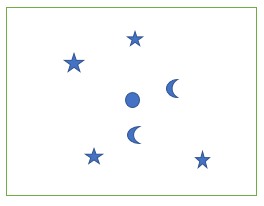
\includegraphics[scale=.5]{Images/KNN}
    \end{center}
    \caption{Ví dụ K-NN}
    \end{figure}
\end{center}
Trong hình 2.13, Training Data là các hình ngôi sao và mặt trăng, hình tròn ở dây là đối tượng cần để xác định lớp (Query Point). Nhiệm vụ của chúng ta là dự đoán lớp của Query Point dựa vào việc lựa chọn số láng giềng gần nhất với nó.\\Ta thấy rằng, với:
\begin{itemize}
\item[•] 1-Nearest Neighbour: Kết quả sẽ là mặt trăng.
\item[•] 4-Nearest Neighbour: Kết quả sẽ không xác định được lớp cho Query Point vì số láng giềng gần nhất với nó là 4 trong đó có 2 cặp đối tượng thuộc 2 lớp khác nhau.
\item[•] 6-Nearest Neighbour: Kết quả sẽ là ngôi sao vì trong 6 láng giềng gần nhất với nó thì có 4 đối tượng thuộc lớp ngôi sao. 
\end{itemize}
\subsection{Thư viện OpenCV}
OpenCV (Open Computer Vision) là một thư viện mã nguồn mở chuyên dùng để xử lý các vấn đề liên quan đến thị giác máy tính. Nhờ một hệ thống các giải thuật chuyên biệt, tối ưu cho việc xử lý thị giác máy tính, vì vậy tính ứng dụng của OpenCV là rất lớn, có thể kể đến như:
\begin{itemize}
\item Nhận dạng ảnh: nhận dạng khuôn mặt, các vật thể, ...
\item Xử lý ảnh: khử nhiễu, điều chỉnh độ sáng, ...
\item Nhận dạng cử chỉ.
\item Và còn nhiều ứng dụng khác nữa.
\end{itemize}
Ta có thể sử dụng nhiều ngôn ngữ lập trình khác nhau để làm việc với OpenCV như C++, Java, Python, CSharp ... \\Ở đồ án này sử dụng OpenCV 4.1.0 trên ngôn ngữ Python 3.7
\section{THIẾT KẾ VÀ THỰC HIỆN CHƯƠNG TRÌNH}
\subsection{Yêu cầu đặt ra}
\begin{itemize}
\item Nhận dạng và phân loại trái Sơri với độ chính xác cao (trên 90 phần trăm).
\item Thời gian nhận dạng và phân loại một trái dưới 0.5 giây.
\end{itemize}
\subsection{Chuẩn bị}
\begin{itemize}
\item Trước tiên cần tiến hành thu thập ảnh để làm Training Data.
\item Để dễ dàng phát hiện được trái Sơri, ở đây trái Sơri được đặt trên nền đen.
\end{itemize}
\subsection{Huấn luyện Haar Cascade [3, 4]}
Tiến hành huấn luyện với 1510 ảnh dương (chứa trái Sơri) và 3000 ảnh âm (không chứa trái Sơri).\\OpenCV cung cấp hai hàm để tiến hành huấn luyện:
\begin{itemize}
\item[•] Sử dụng \textbf{opencv-createsamples.exe} để tạo ra file vector chứa các mẫu huấn luyện
\begin{center}
    \begin{figure}[htp]
    \begin{center}
    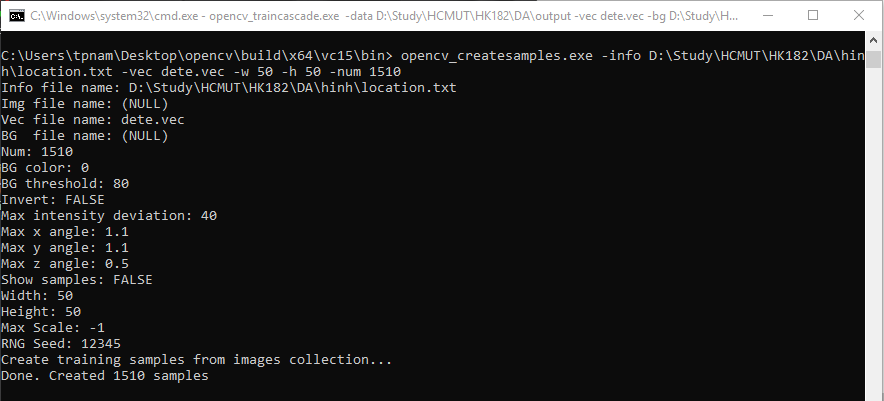
\includegraphics[scale=.7]{Images/vector}
    \end{center}
    \caption{Tạo file vector chứa ảnh huấn luyện}
    \end{figure}
\end{center}
\pagebreak
\item[•] Sử dụng \textbf{opencv-traincascade.exe} lấy ảnh trong file vector đặt ngẫu nhiên vào các ảnh âm để rút trích đặc trưng.
\begin{center}
    \begin{figure}[htp]
    \begin{center}
    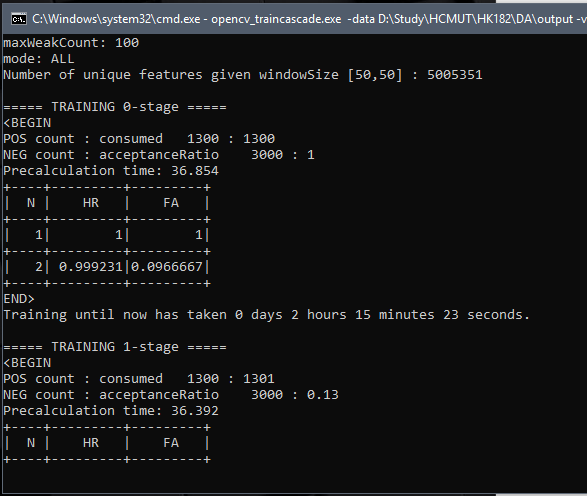
\includegraphics[scale=.7]{Images/train}
    \end{center}
    \caption{Qúa trình huấn luyện}
    \end{figure}
\end{center}
\item[•] Sau khi huấn luyện ta sẽ được file \textbf{cascade.xml} chứa các ngưỡng và đặc trưng trong các bộ phân loại yếu. Sử dụng file xml này để sử dụng cho chương trình chính.
\end{itemize}
\pagebreak
\subsection{Tìm đặc trưng cho việc huấn luyện K-NN}
Như đã nói ở phần lý thuyết, mỗi một điểm ảnh trên một bức ảnh được biểu diễn bỏi 3 giá trị kênh màu RGB. Tiến hành lấy trung bình cộng giá trị 3 kênh màu trên 100 ảnh trái chín và 100 trái xanh ta thu được kết quả sau:
\begin{center}
	\begin{table}[htp]
		\begin{center}
		\begin{tabular}{|c|c|c|c|c|c|c|}
		\hline
		STT & \multicolumn{3}{|c|}{Trái xanh} & \multicolumn{3}{|c|}{Trái chín}\\
		\hline
		  & B & G & R & B & G & R\\
		\hline
		1 & 8.2 & 47.4 & 31.0 & 37.3 & 46.6 & 98.4\\
		2 & 22.1 & 108.3 & 103.7 & 41.5 & 44.7 & 80.2\\
		3 & 19.6 & 90.0 & 76.2 & 36.4 & 45.5 & 79.5\\
		4 & 22.9 & 71.3 & 71.4 & 42.5 & 50.3 & 84.3\\
		5 & 21.3 & 91.5 & 101.9 & 45.4 & 68.2 & 120.9\\
		6 & 28.5 & 74.6 & 75.4 & 34.5 & 36.9 & 75.8\\
		7 & 24.1 & 96.6 & 100.4 & 42.4 & 61.7 & 89.3\\
		8 & 24.2 & 69.5 & 67.0 & 62.5 & 81.5 & 113.2\\
		9 & 14.7 & 68.6 & 74.1 & 34.1 & 40.9 & 78.0\\
		10 & 22.9 & 71.1 & 63.3 & 39.4 & 40.9 & 89.1\\
		... & ... & ... & ... & ... & ... & ...\\
		\hline
		Trung bình & 41.4 & 85 & 81.3 & 40.0 & 57.4 & 109.9\\
		\hline
		\end{tabular}
		\begin{center}
		\caption{Bảng giá trị trung bình các kênh màu trên trái Xanh và Chín}
		\end{center}
		\end{center}
	\end{table}
\end{center}
Dựa vào bảng trên ta có thể thấy tỷ lệ giữa kênh màu G và R giữa trái xanh và trái chín có sự khác biệt khá rõ rệt nên ta sẽ chọn làm đặc trưng.
\subsection{Sơ đồ khối}
\begin{center}
    \begin{figure}[htp]
    \begin{center}
    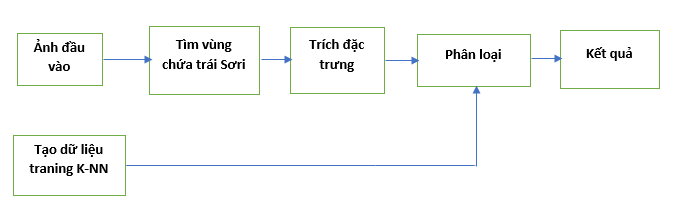
\includegraphics[scale=.8]{Images/blockKNN}
    \end{center}
    \caption{Sơ đồ khối}
    \end{figure}
\end{center}
\pagebreak
\subsubsection{Ảnh đầu vào}
Chụp từ Webcam (Logitech C270) độ phân giải 640x480 pixels, trái Sơri đặt trên nền tối màu, không để các nguồn sáng ảnh hưởng đến hình ảnh thu được.
\subsubsection{Dữ liệu Training K-NN}
Được lấy từ 900 trái chín và 900 trái xanh khác nhau. Tiến hành lấy trung bình giá trị kênh màu G và R của từng ảnh, sau đó ghép lại thành một vector đặc trưng lớn. Sử dụng hàm \textbf{cv2.ml.KNearest-create()} do OpenCV cung cấp để tạo ra bộ phân loại. Do thuật toán Haar và Adaboost chỉ làm việc trên ảnh xám nên ta dùng hàm \textbf{cv2.cvtColor(image, cv2.COLOR-BGR2GRAY)}để chuyển ảnh này sang ảnh xám.
\subsubsection{Tìm vùng chứa trái Sơri}
Từ dữ liệu đầu vào, sử sụng file cascade.xml có được sau huấn luyện Haar Cascade để tìm vùng chứa trái Sơri. Để phát hiện trái Sơri, hệ thống sẽ cho một cửa sổ con(sub-window) có kích thước cố định quét lên toàn bộ ảnh đầu vào. Như vậy sẽ có rất nhiều ảnh con ứng với từng cửa sổ con, các đặc trưng Haar-like sẽ được đặc lên các cửa sổ con này để từ đó tính ra giá trị của đặc trưng. Sau đó các giá trị này được bộ phân loại xác nhận xem khung hình đó có phải trái Sơri hay không. OpenCV cung cấp sẵn một số hàm hỗ trợ cho việc này:\\
\begin{itemize}
\item[-] \textbf{cv2.CascadeClassifier("file.xml")} : Hàm này khai báo file xml
\item[-] \textbf{detectMultiScale(image, ScaleFactor, minNeighbours)}: Hàm này sẽ phát hiện vùng chứa trái Sơri có trong ảnh, trả về các giá trị tọa độ và độ rộng, độ cao của vùng, nhờ đó ta có thể vẽ được khung chứa trái Sơri.
\begin{itemize}
\item[•] \textbf{image}: ảnh đầu vào.
\item[•] \textbf{ScaleFactor}: Tỷ lệ tăng kích thước của khung cửa sổ tìm kiếm.Ví dụ nếu ScaleFactor=1.1 thì sau khi quét hết bức ảnh 1 lần, khung cửa sổ sẽ tăng kich thước lên 10 phần trăm và thực hiện lần quét tiếp theo. Tham số này ảnh hưởng đến tốc độ xử lý và độ tin cậy của chương trình. Nếu để nó quá lớn thì tốc độ chương trình sẽ tăng lên do số lần quét giảm đi, tuy nhiên có thể chương trình có thể bỏ qua không phát hiện được một số trái có kích thước nằm giữa 2 khung cửa sổ liên tiếp do độ tăng kích thước của khung là quá lớn. Nếu để nó quá thấp thì ta có thể không bỏ sót bất kì trái nào nhưng chương trình sẽ tốn thời gian hơn vì tăng số lần quét lên.
\pagebreak
\item[•] \textbf{minNeighbour}: giá trị tối thiểu số hình chữ nhật lân cận được gộp lại sau khi quá trình quét đã xong. Trong quá trình tìm kiếm trái Sơri chương trình sẽ tìm được nhiều những khung hình chữ nhật chứa trái Sơri cho dù đó chỉ là một trái và có nhưng trường hợp nhận diện nhầm.\\Nếu ta để minNeighbour = 0 kết quả sẽ cho ra:
\begin{center}
    \begin{figure}[htp]
    \begin{center}
    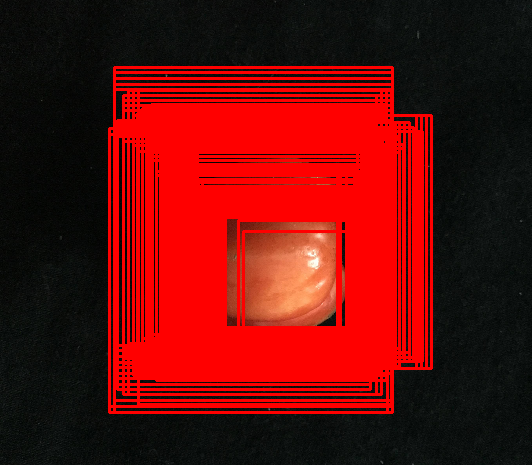
\includegraphics[scale=.4]{Images/zero}
    \end{center}
    \caption{minNeighbour = 0}
    \end{figure}
\end{center}
Còn khi cho minNeighbour = 5 kết quả sẽ là:
\begin{center}
    \begin{figure}[htp]
    \begin{center}
    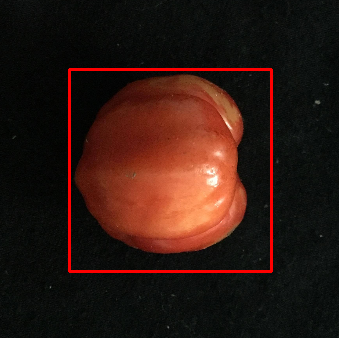
\includegraphics[scale=.4]{Images/five}
    \end{center}
    \caption{minNeighbour = 5}
    \end{figure}
\end{center}
\end{itemize}
\end{itemize}
\subsubsection{Trích đặc trưng}
Sau khi xác định được khu vực nào chứa trái Sơri, tiến hành tính trung bình giá trị kênh màu G và R của vùng đó để làm vector đặc trưng.
\subsubsection{Phân loại}
Sau khi đã có được đặc trưng của trái Sơri cần phân loại, sử dụng hàm \textbf{findNearest(đặc trưng của trái cần phân loại, số láng giềng gần nhất)} do OpenCV cung cấp để dự đoán kết quả.
\pagebreak
\section{KẾT QUẢ THỰC HIỆN}
\subsection{Tiến hành thực nghiệm}
Tiến hành thực nghiệm trên 350 mẫu xanh và 350 mẫu chín (mỗi ảnh chứa một trái, không bao gồm các ảnh đã huấn luyện). Sơri được đặt trên nền đen, chụp bằng webcam (640x480 pixels). K láng giềng tăng dần từ 1 đến 20, sacleFactor là 1.2, minNeighbour là 10.
\subsection{Kết quả thu được sau thực nghiệm}
Kết quả với K-láng giềng bằng 1.
\begin{center}
	\begin{table}[htp]
	\begin{center}
	\begin{tabular}{|c|c|c|c|c|c|}
	\hline
	\multicolumn{3}{|c|}{Trái xanh} & \multicolumn{3}{|c|}{Trái chín}\\
	\hline
	Detected & Phân loại đúng & Phân loại sai & Detected & Phân loại đúng & Phân loại sai\\
	\hline
	300 & 334 & 16 & 300 & 341 & 9\\
	\hline 
	\end{tabular}
	\begin{center}
	\caption{Kết quả nhận dạng với K = 1}
	\end{center}
	\end{center}
	\end{table}
\end{center}

Tỷ lệ nhận dạng chính xác: \textbf{92.9} phần trăm.

Thời gian nhận dạng và phân loại một trái: 0.0346 giây.


Kết quả với K-láng giềng bằng 5
\begin{center}
	\begin{table}[htp]
	\begin{center}
	\begin{tabular}{|c|c|c|c|c|c|}
	\hline
	\multicolumn{3}{|c|}{Trái xanh} & \multicolumn{3}{|c|}{Trái chín}\\
	\hline
	Detected & Phân loại đúng & Phân loại sai & Detected & Phân loại đúng & Phân loại sai\\
	\hline
	300 & 338 & 12 & 300 & 342 & 8\\
	\hline 
	\end{tabular}
	\begin{center}
	\caption{Kết quả nhận dạng với K = 5}
	\end{center}
	\end{center}
	\end{table}
\end{center}

Tỷ lệ nhận dạng chính xác: \textbf{94.4} phần trăm.

Thời gian nhận dạng và phân loại một trái: 0.055 giây.

Tăng thêm K thì Tỷ lệ chính xác vẫn không tăng thêm, thời gian nhận dạng và phân loại tăng.

\pagebreak
Một số hình ảnh thu được:
\begin{center}
    \begin{figure}[htp]
    \begin{center}
    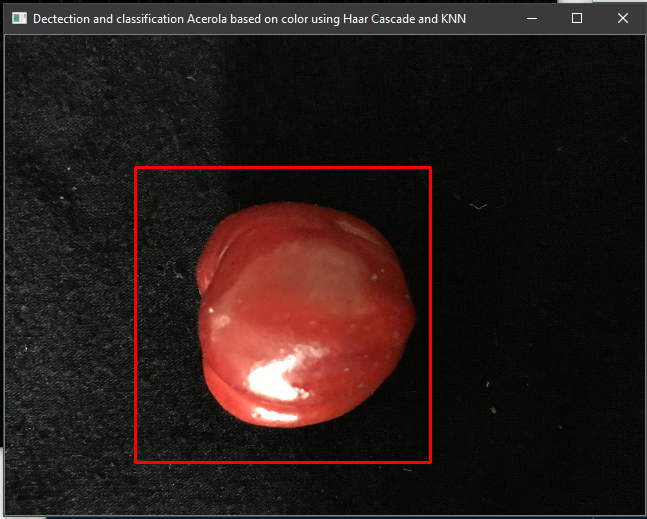
\includegraphics[scale=.4]{Images/f1}
    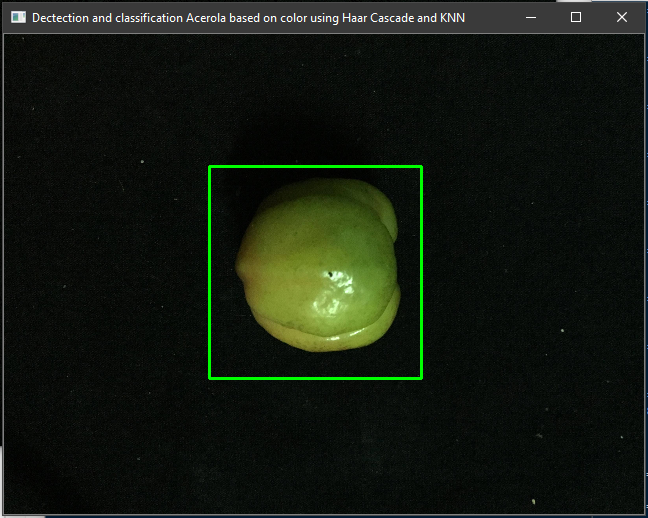
\includegraphics[scale=.4]{Images/f3}
    \end{center}
    \caption{Kết quả với một trái trên hình}
    \end{figure}
\end{center}
\begin{center}
    \begin{figure}[htp]
    \begin{center}
    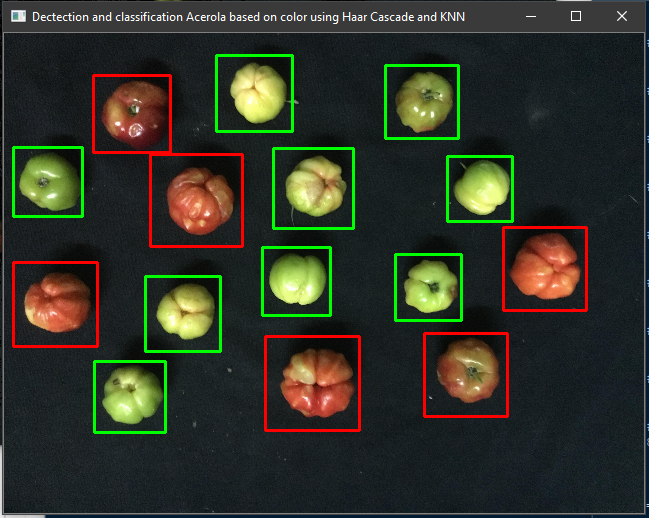
\includegraphics[scale=.8]{Images/f2}
    \end{center}
    \caption{Kết quả với nhiều trái trên hình}
    \end{figure}
\end{center}
\pagebreak
\subsection{Giải thích và phân tích kết quả}
\begin{itemize}
\item[-] Kết quả thu được cho thấy chương trình thực hiện khá tốt. Tỷ lệ chính xác còn tùy thuộc vào số K láng giềng tuy nhiên không ảnh hưởng nhiều do số lượng dữ liệu tham chiếu khá lớn. Thời gian nhận dạng và phân loại khá nhanh do ảnh có độ phân giải thấp (640x480 pixels) và giá scaleFactor lớn (1.2)
\item[-] Một số trái phân loại chưa chính xác do các nguyên nhân sau:
\begin{itemize}
\item[•] Dữ liệu sử dụng làm mẫu huấn luyện chưa chuẩn. Do được chọn lọc thủ công nên trong quá trình phân loại không tránh khỏi sai sót, mang yếu tố chủ quan.
\item[•] Một số trái không chín hẳn cũng không xanh hẳn, điều này dẫn đến kết quả sẽ phụ thuộc vào góc chụp.
\begin{center}
    \begin{figure}[htp]
    \begin{center}
    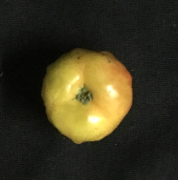
\includegraphics[scale=.8]{Images/tren}
    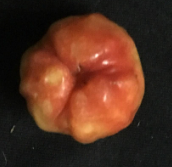
\includegraphics[scale=.8]{Images/duoi}
    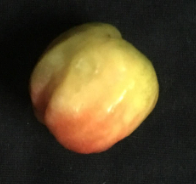
\includegraphics[scale=.8]{Images/ngang}
    \end{center}
    \caption{3 mặt của cùng một trái Sơri bị phân loại sai}
    \end{figure}
\end{center}
\end{itemize}
\end{itemize}
\section{KẾT LUẬN VÀ HƯỚNG PHÁT TRIỂN}
\subsection{Kết luận}
\begin{itemize}
\item[-] Kết quả thu được đáp ứng được mục tiêu đề ra ban đầu (nhận dạng đúng trên 90 phần trăm) thời gian nhận dạng và phân loại nhanh (nhỏ hơn 0.5 giây).
\item[-] Để có được kết quả tốt nhất, cần phải chuẩn bị dữ liệu huấn luyện thật chuẩn, nhiều.
\item[-] Điều kiện chụp: tránh ảnh hưởng của các nguồn sáng đến màu sắc của trái Sơri.
\end{itemize}
\subsection{Hướng phát triển}
\begin{itemize}
\item[-] Phát triển thêm để có thể nhận diện được các trái hư (hỏng).
\item[-] Kết hợp với phần cứng để tạo thành hệ thống phân loại hoàn chỉnh.  
\end{itemize}
\pagebreak
\section{TÀI LIỆU THAM KHẢO}
[1] Paul Viola and Michael Jones, Rapid Object Detection using a Boosted Cascade of Simple Features, 2001.

[2] Cascade classifier class for object detection, https://docs.opencv.org/3.4/d1/de5/classcv-1-1CascadeClassifier.html

[3] Train a Cascade Object Detector, https://www.mathworks.com/help/vision/ug/train-a-cascade-object-detector.html

[4] Phát hiện đối tượng, https://thigiacmaytinh.com/phat-hien-doi-tuong-p1-ly-thuyet/ 

[5] The OpenCV Tutorials Release 2.4.13.7

[6] Vũ Hữu Tiệp, K-nearest neighbors, https://machinelearningcoban.com/2017/01/08/knn/
\pagebreak
\section{PHỤ LỤC}
Toàn bộ chương trình:
\begin{lstlisting}
import numpy as np
import cv2

pathR = 'D:/Study/HCMUT/HK182/DA/Images/Samples/2Color/Red/'
pathG = 'D:/Study/HCMUT/HK182/DA/Images/Samples/2Color/Green/'

size = 20
train_ids = np.arange(1, 901)


def buildfilename(path, pre, im_ids):
    filename = []
    for im_id in im_ids:
        fn = path + pre + '-' + str(im_id) + '.png'
        filename.append(fn)
    return filename


def resize(filename):
    img = cv2.imread(filename)
    img = cv2.resize(img, (size, size))
    return img


def trainsamples(img_ids):
    filenamegreen = buildfilename(pathG, 'G', img_ids)
    filenamered = buildfilename(pathR, 'R', img_ids)
    filenamefull = filenamegreen + filenamered
    resized = []
    feature = []
    for i in range(len(filenamefull)):
        x = resize(filenamefull[i])
        resized.append(x)
    for i in range(len(resized)):
        x = resized[i]
        f = []
        # blue = 0
        green = 0
        red = 0
        for j in range(len(x)):
            cell = x[j]
            for z in range(len(cell)):
                # blue = blue + cell[j][0]
                green = green + cell[j][1]
                red = red + cell[j][2]
        # f.append(int(blue/(size*size)))
        f.append(int(green / (size * size)))
        f.append(int(red / (size * size)))
        feature.append(f)
    feature = np.array(feature).astype(np.float32)
    return feature


x = trainsamples(train_ids)
k = np.arange(2)
lable = np.repeat(k, len(x) / 2)[:, np.newaxis]
knn = cv2.ml.KNearest_create()
knn.train(x, 0, lable)


def test(filename):
    f = []
    t = []
    img = cv2.imread(filename)
    img = cv2.resize(img, (size, size))
    # blue = 0
    green = 0
    red = 0
    for i in range(len(img)):
        cell = img[i]
        for j in range(len(cell)):
            # blue = blue + cell[j][0]
            green = green + cell[j][1]
            red = red + cell[j][2]
    # f.append(int(blue/(size*size)))
    f.append(int(green / (size * size)))
    f.append(int(red / (size * size)))
    t.append(f)
    sp = np.array(t).astype(np.float32)
    kq1, kq2, kq3, kq4 = knn.findNearest(sp, 20)
    return kq2

soridetect = cv2.CascadeClassifier("cascade1.xml")

cap = cv2.VideoCapture(1)

while True:
    ret, frame = cap.read()
    if ret != 1:
        print("Video finished")
        break
    frame = cv2.resize(frame, (640, 480))
    gray = cv2.cvtColor(frame, cv2.COLOR_BGR2GRAY)
    sori = soridetect.detectMultiScale(
        gray,
        scaleFactor=1.2,
        minNeighbors=10,
    )
    for (x, y, w, h) in sori:
        img_crop = frame[y + 2:y + h - 2, x + 2:x + w - 2, :]
        cv2.imwrite('object.jpg', img_crop)
        c = test('object.jpg')
        font = cv2.FONT_HERSHEY_SIMPLEX
        if c == 0:
            cv2.rectangle(frame, (x, y), (x + w, y + h), (0, 255, 0), 2)
            # cv2.putText(frame, 'xanh', (x, y - 5), font, 0.5, (0, 255, 0), 1, cv2.LINE_AA)
        else:
            cv2.rectangle(frame, (x, y), (x + w, y + h), (0, 0, 255), 2)
            # cv2.putText(frame, 'chin', (x, y - 5), font, 0.5, (0, 255, 0), 1, cv2.LINE_AA)
    cv2.imshow('Dectection and classification Acerola based on color using Haar Cascade and KNN', frame)
    if cv2.waitKey(1) == 27:
        print('Bye bye !!!')
        break
cap.release()
cv2.destroyAllWindows()
\end{lstlisting}
\end{document}